\documentclass{beamer}

\usetheme{Warsaw}
\usepackage{graphicx}
\usepackage{ulem}
\usepackage{tikz}
\usepackage{cancel}
% include.tex
\newcommand{\Bernoulli}[1]{\text{Bernoulli} \left( #1 \right)}
\newcommand{\mydigamma}[1]{\psi \left( #1 \right)}
%\newcommand{\diag}[1]{\text{diag}\left( #1 \right)}
\newcommand{\tr}[1]{\text{tr}\left( #1 \right)}
\newcommand{\Poisson}[1]{\text{Poisson} \left( #1 \right)}
\def \half {\frac{1}{2}}
\def \R {\mathbb{R}}
\def \vbeta {\vec{\beta}}
\def \vy {\vec{y}}
\def \vmu {\vec{\mu}}
\def \vmuqbeta {\vmu_{q(\vbeta)}}
\def \vmubeta {\vmu_{\vbeta}}
\def \Sigmaqbeta {\Sigma_{q(\vbeta)}}
\def \Sigmabeta {\Sigma_{\vbeta}}
\def \va {\vec{a}}
\def \vtheta {\vec{\theta}}
\def \mX {\vec{X}}

\def\ds{{\displaystyle}}

\def\diag{{\mbox{diag}}}


\usepackage{latexsym,amssymb,amsmath,amsfonts}
%\usepackage{tabularx}
\usepackage{theorem}
\usepackage{verbatim,array,multicol,palatino}
\usepackage{graphicx}
\usepackage{graphics}
\usepackage{fancyhdr}
\usepackage{algorithm,algorithmic}
\usepackage{url}
%\usepackage[all]{xy}



\def\approxdist{\stackrel{{\tiny \mbox{approx.}}}{\sim}}
\def\smhalf{\textstyle{\frac{1}{2}}}
\def\vxnew{\vx_{\mbox{{\tiny new}}}}
\def\bib{\vskip12pt\par\noindent\hangindent=1 true cm\hangafter=1}
\def\jump{\vskip3mm\noindent}
\def\etal{{\em et al.}}
\def\etahat{{\widehat\eta}}
\def\thick#1{\hbox{\rlap{$#1$}\kern0.25pt\rlap{$#1$}\kern0.25pt$#1$}}
\def\smbbeta{{\thick{\scriptstyle{\beta}}}}
\def\smbtheta{{\thick{\scriptstyle{\theta}}}}
\def\smbu{{\thick{\scriptstyle{\rm u}}}}
\def\smbzero{{\thick{\scriptstyle{0}}}}
\def\boxit#1{\begin{center}\fbox{#1}\end{center}}
\def\lboxit#1{\vbox{\hrule\hbox{\vrule\kern6pt
      \vbox{\kern6pt#1\kern6pt}\kern6pt\vrule}\hrule}}
\def\thickboxit#1{\vbox{{\hrule height 1mm}\hbox{{\vrule width 1mm}\kern6pt
          \vbox{\kern6pt#1\kern6pt}\kern6pt{\vrule width 1mm}}
               {\hrule height 1mm}}}


%\sloppy
%\usepackage{geometry}
%\geometry{verbose,a4paper,tmargin=20mm,bmargin=20mm,lmargin=40mm,rmargin=20mm}


%%%%%%%%%%%%%%%%%%%%%%%%%%%%%%%%%%%%%%%%%%%%%%%%%%%%%%%%%%%%%%%%%%%%%%%%%%%%%%%%
%
% Some convenience definitions
%
% \bf      -> vector
% \sf      -> matrix
% \mathcal -> sets or statistical
% \mathbb  -> fields or statistical
%
%%%%%%%%%%%%%%%%%%%%%%%%%%%%%%%%%%%%%%%%%%%%%%%%%%%%%%%%%%%%%%%%%%%%%%%%%%%%%%%%

% Sets or statistical values
\def\sI{{\mathcal I}}                            % Current Index set
\def\sJ{{\mathcal J}}                            % Select Index set
\def\sL{{\mathcal L}}                            % Likelihood
\def\sl{{\ell}}                                  % Log-likelihood
\def\sN{{\mathcal N}}                            
\def\sS{{\mathcal S}}                            
\def\sP{{\mathcal P}}                            
\def\sQ{{\mathcal Q}}                            
\def\sB{{\mathcal B}}                            
\def\sD{{\mathcal D}}                            
\def\sT{{\mathcal T}}
\def\sE{{\mathcal E}}                            
\def\sF{{\mathcal F}}                            
\def\sC{{\mathcal C}}                            
\def\sO{{\mathcal O}}                            
\def\sH{{\mathcal H}} 
\def\sR{{\mathcal R}}                            
\def\sJ{{\mathcal J}}                            
\def\sCP{{\mathcal CP}}                            
\def\sX{{\mathcal X}}                            
\def\sA{{\mathcal A}} 
\def\sZ{{\mathcal Z}}                            
\def\sM{{\mathcal M}}                            
\def\sK{{\mathcal K}}     
\def\sG{{\mathcal G}}                         
\def\sY{{\mathcal Y}}                         
\def\sU{{\mathcal U}}  


\def\sIG{{\mathcal IG}}                            


\def\cD{{\sf D}}
\def\cH{{\sf H}}
\def\cI{{\sf I}}

% Vectors
\def\vectorfontone{\bf}
\def\vectorfonttwo{\boldsymbol}
\def\va{{\vectorfontone a}}                      %
\def\vb{{\vectorfontone b}}                      %
\def\vc{{\vectorfontone c}}                      %
\def\vd{{\vectorfontone d}}                      %
\def\ve{{\vectorfontone e}}                      %
\def\vf{{\vectorfontone f}}                      %
\def\vg{{\vectorfontone g}}                      %
\def\vh{{\vectorfontone h}}                      %
\def\vi{{\vectorfontone i}}                      %
\def\vj{{\vectorfontone j}}                      %
\def\vk{{\vectorfontone k}}                      %
\def\vl{{\vectorfontone l}}                      %
\def\vm{{\vectorfontone m}}                      % number of basis functions
\def\vn{{\vectorfontone n}}                      % number of training samples
\def\vo{{\vectorfontone o}}                      %
\def\vp{{\vectorfontone p}}                      % number of unpenalized coefficients
\def\vq{{\vectorfontone q}}                      % number of penalized coefficients
\def\vr{{\vectorfontone r}}                      %
\def\vs{{\vectorfontone s}}                      %
\def\vt{{\vectorfontone t}}                      %
\def\vu{{\vectorfontone u}}                      % Penalized coefficients
\def\vv{{\vectorfontone v}}                      %
\def\vw{{\vectorfontone w}}                      %
\def\vx{{\vectorfontone x}}                      % Covariates/Predictors
\def\vy{{\vectorfontone y}}                      % Targets/Labels
\def\vz{{\vectorfontone z}}                      %

\def\vone{{\vectorfontone 1}}
\def\vzero{{\vectorfontone 0}}

\def\valpha{{\vectorfonttwo \alpha}}             %
\def\vbeta{{\vectorfonttwo \beta}}               % Unpenalized coefficients
\def\vgamma{{\vectorfonttwo \gamma}}             %
\def\vdelta{{\vectorfonttwo \delta}}             %
\def\vepsilon{{\vectorfonttwo \epsilon}}         %
\def\vvarepsilon{{\vectorfonttwo \varepsilon}}   % Vector of errors
\def\vzeta{{\vectorfonttwo \zeta}}               %
\def\veta{{\vectorfonttwo \eta}}                 % Vector of natural parameters
\def\vtheta{{\vectorfonttwo \theta}}             % Vector of combined coefficients
\def\vvartheta{{\vectorfonttwo \vartheta}}       %
\def\viota{{\vectorfonttwo \iota}}               %
\def\vkappa{{\vectorfonttwo \kappa}}             %
\def\vlambda{{\vectorfonttwo \lambda}}           % Vector of smoothing parameters
\def\vmu{{\vectorfonttwo \mu}}                   % Vector of means
\def\vnu{{\vectorfonttwo \nu}}                   %
\def\vxi{{\vectorfonttwo \xi}}                   %
\def\vpi{{\vectorfonttwo \pi}}                   %
\def\vvarpi{{\vectorfonttwo \varpi}}             %
\def\vrho{{\vectorfonttwo \rho}}                 %
\def\vvarrho{{\vectorfonttwo \varrho}}           %
\def\vsigma{{\vectorfonttwo \sigma}}             %
\def\vvarsigma{{\vectorfonttwo \varsigma}}       %
\def\vtau{{\vectorfonttwo \tau}}                 %
\def\vupsilon{{\vectorfonttwo \upsilon}}         %
\def\vphi{{\vectorfonttwo \phi}}                 %
\def\vvarphi{{\vectorfonttwo \varphi}}           %
\def\vchi{{\vectorfonttwo \chi}}                 %
\def\vpsi{{\vectorfonttwo \psi}}                 %
\def\vomega{{\vectorfonttwo \omega}}             %


% Matrices
%\def\matrixfontone{\sf}
%\def\matrixfonttwo{\sf}
\def\matrixfontone{\bf}
\def\matrixfonttwo{\boldsymbol}
\def\mA{{\matrixfontone A}}                      %
\def\mB{{\matrixfontone B}}                      %
\def\mC{{\matrixfontone C}}                      % Combined Design Matrix
\def\mD{{\matrixfontone D}}                      % Penalty Matrix for \vu_J
\def\mE{{\matrixfontone E}}                      %
\def\mF{{\matrixfontone F}}                      %
\def\mG{{\matrixfontone G}}                      % Penalty Matrix for \vu
\def\mH{{\matrixfontone H}}                      %
\def\mI{{\matrixfontone I}}                      % Identity Matrix
\def\mJ{{\matrixfontone J}}                      %
\def\mK{{\matrixfontone K}}                      %
\def\mL{{\matrixfontone L}}                      % Lower bound
\def\mM{{\matrixfontone M}}                      %
\def\mN{{\matrixfontone N}}                      %
\def\mO{{\matrixfontone O}}                      %
\def\mP{{\matrixfontone P}}                      %
\def\mQ{{\matrixfontone Q}}                      %
\def\mR{{\matrixfontone R}}                      %
\def\mS{{\matrixfontone S}}                      %
\def\mT{{\matrixfontone T}}                      %
\def\mU{{\matrixfontone U}}                      % Upper bound
\def\mV{{\matrixfontone V}}                      %
\def\mW{{\matrixfontone W}}                      % Variance Matrix i.e. diag(b'')
\def\mX{{\matrixfontone X}}                      % Unpenalized Design Matrix/Nullspace Matrix
\def\mY{{\matrixfontone Y}}                      %
\def\mZ{{\matrixfontone Z}}                      % Penalized Design Matrix/Kernel Space Matrix

\def\mGamma{{\matrixfonttwo \Gamma}}             %
\def\mDelta{{\matrixfonttwo \Delta}}             %
\def\mTheta{{\matrixfonttwo \Theta}}             %
\def\mLambda{{\matrixfonttwo \Lambda}}           % Penalty Matrix for \vnu
\def\mXi{{\matrixfonttwo \Xi}}                   %
\def\mPi{{\matrixfonttwo \Pi}}                   %
\def\mSigma{{\matrixfonttwo \Sigma}}             %
\def\mUpsilon{{\matrixfonttwo \Upsilon}}         %
\def\mPhi{{\matrixfonttwo \Phi}}                 %
\def\mOmega{{\matrixfonttwo \Omega}}             %
\def\mPsi{{\matrixfonttwo \Psi}}                 %

\def\mone{{\matrixfontone 1}}
\def\mzero{{\matrixfontone 0}}

% Fields or Statistical
\def\bE{{\mathbb E}}                             % Expectation
\def\bP{{\mathbb P}}                             % Probability
\def\bR{{\mathbb R}}                             % Reals
\def\bI{{\mathbb I}}                             % Reals
\def\bV{{\mathbb V}}                             % Reals

\def\vX{{\vectorfontone X}}                      % Targets/Labels
\def\vY{{\vectorfontone Y}}                      % Targets/Labels
\def\vZ{{\vectorfontone Z}}                      %

% Other
\def\etal{{\em et al.}}
\def\ds{\displaystyle}
\def\d{\partial}
\def\diag{\text{diag}}
%\def\span{\text{span}}
\def\blockdiag{\text{blockdiag}}
\def\tr{\text{tr}}
\def\RSS{\text{RSS}}
\def\df{\text{df}}
\def\GCV{\text{GCV}}
\def\AIC{\text{AIC}}
\def\MLC{\text{MLC}}
\def\mAIC{\text{mAIC}}
\def\cAIC{\text{cAIC}}
\def\rank{\text{rank}}
\def\MASE{\text{MASE}}
\def\SMSE{\text{SASE}}
\def\sign{\text{sign}}
\def\card{\text{card}}
\def\notexp{\text{notexp}}
\def\ASE{\text{ASE}}
\def\ML{\text{ML}}
\def\nullity{\text{nullity}}

\def\logexpit{\text{logexpit}}
\def\logit{\mbox{logit}}
\def\dg{\mbox{dg}}

\def\Bern{\mbox{Bernoulli}}
\def\sBernoulli{\mbox{Bernoulli}}
\def\sGamma{\mbox{Gamma}}
\def\sInvN{\mbox{Inv}\sN}
\def\sNegBin{\sN\sB}

\def\dGamma{\mbox{Gamma}}
\def\dInvGam{\mbox{Inv}\Gamma}

\def\Cov{\mbox{Cov}}
\def\Mgf{\mbox{Mgf}}

\def\mis{{mis}} 
\def\obs{{obs}}

\def\argmax{\operatornamewithlimits{\text{argmax}}}
\def\argmin{\operatornamewithlimits{\text{argmin}}}
\def\argsup{\operatornamewithlimits{\text{argsup}}}
\def\arginf{\operatornamewithlimits{\text{arginf}}}


\def\minimize{\operatornamewithlimits{\text{minimize}}}
\def\maximize{\operatornamewithlimits{\text{maximize}}}
\def\suchthat{\text{such that}}


\def\relstack#1#2{\mathop{#1}\limits_{#2}}
\def\sfrac#1#2{{\textstyle{\frac{#1}{#2}}}}


\def\comment#1{
\vspace{0.5cm}
\noindent \begin{tabular}{|p{14cm}|}  
\hline #1 \\ 
\hline 
\end{tabular}
\vspace{0.5cm}
}


\def\mytext#1{\begin{tabular}{p{13cm}}#1\end{tabular}}
\def\mytextB#1{\begin{tabular}{p{7.5cm}}#1\end{tabular}}
\def\mytextC#1{\begin{tabular}{p{12cm}}#1\end{tabular}}

\def\jump{\vskip3mm\noindent}

\def\KL{\text{KL}}
\def\N{\text{N}}
\def\Var{\text{Var}}

\def \E {\mathbb{E}}
\def \BigO {\text{O}}
\def \IG {\text{IG}}
\def \Beta {\text{Beta}}



\usefonttheme{serif}

\title{How I learned to stop worrying and love floating point numbers.}
\author{Mark Greenaway \\ PhD candidate \\ markg@maths.usyd.edu.au}

% \usetikzlibrary{arrows.meta}
% \directlua{
% function f(x) 
%   return x / (1 + abs(x))
% end
% }
% \pgfmathdeclarefunction{Unum_function}{1}{%
%   \edef\pgfmathresult{%
%      \directlua{tex.print("" .. f(#1))}%
%    }%  
% }

\mode<presentation>
{ \usetheme{boxes} }

\begin{document}
\begin{frame}
\maketitle
\end{frame}

% Abstract:

% In this talk we will construct the natural numbers, the integers and the rational numbers. We will then
% discuss the fact that the rational numbers are not complete, but have ``holes'', motivating the construction
% of the real numbers. It will be shown that while the rational numbers are countable, the real numbers are not.
% This forces us to approximate if we wish to perform calculations on a finite memory computer in finite time.

% The three major approaches to this problem will be introduced - fixed point, floating point and arbitrary
% precision. Of these, floating point is the one most programmers are likely to first encounter, and the one
% implemented in hardware that you can actually buy today. We will discuss the floating point numbers, along
% with the implications of their definition using some elementary results from numerical analysis. We will also
% discuss alternative representations, particularly arbitrary precision, along with their benefits and
% drawbacks. Some interesting work from the Haskell community in this area will be discussed, including recent
% work by Edward Kmett.

% As mathematics is not a spectator sport, all major results will be proven, assuming only the ZFC axioms. This
% talk will be accessible to anyone with a basic knowledge of high school mathematics and an inquiring mind.

\begin{frame}{Who am I?}
\begin{itemize}
\item Third year PhD student working with Dr John Ormerod on variational approximations to Bayesian models.
\item Bachelor Computer Science undergrad at University of Western Sydney.
\item Bachelor of Science in Pure Mathematics and Statistics, First Class Honours, at University of Sydney.
\item Computational statistician.
\item I developed a deep interest in numerical analysis largely out of necessity, because of this darling 
creature
\def \Inf {\text{Inf}}
\def \NaN {\text{NaN}}
\begin{equation*}
\begin{pmatrix}
\Inf & \NaN & \ldots & \NaN\\
\NaN & \Inf & \NaN & \vdots \\
\vdots & \NaN & \ddots & \vdots \\
\NaN & \ldots & \ldots & \Inf
\end{pmatrix}
\end{equation*}
\item He arises when you try to invert a nearly singular matrix. I hope not to meet him again too often in 
			the	near future!
\end{itemize}
\end{frame}

% I want to cover how numbers are constructed, starting from the natural numbers up to the integers, the
% rationals and then the real and complex numbers.

% Because mathematics is \emph{not} a spectator sport, I will be doing this with proofs, live, on the
% whiteboard.

% I'm willing to spend a little bit of time on foundational issues, but not a lot. I'm a mathematical
% analysis/mathematical statistician. There are certain things we accept without question. For instance, most
% mathematicians accept that

% \begin{equation*}
% \mathbb{N} \subset \mathbb{Z} \subset \mathbb{R} \subset \mathbb{C}
% \end{equation*}

% but Liam, Tran's boyfriend, doesn't. He claims that the statement doesn't type check, and hence is
% meaningless. I suspect he's trolling/showing off his superior type theory knowledge, but have been unable to
% pin him down on the issue. Virtually no practicing mathematician would accept this argument. But I'm not a
% type theorist or a Haskell programmer, so my perspective is different. I don't give a flying fuck whether
% things type check, or are even computable. And neither do most pure mathematicians. We work with non-
% computable things all the time. It doesn't trouble us.

% Like the reals. I'm going to present one proof that the reals are uncountable, my favorite one which I learned
% in my third year measure theory course. It's relatively elementary. I'm introducing it because it shows that
% you can't possibly compute with the reals on a computer with finite memory in finite time.

% I'm also going to include a proof that you need the irrational numbers to complete the reals, using the
% square root of 2, although $\pi$ would work just as well.

\begin{frame}{A whirlwind introduction to set theory}
$\forall x$ means for all $x$.\\
To avoid set paradoxes, a set can contain anything except itself.\\
In particular, sets can contain numbers, and other sets.
Infinite sets are fine, whether countably or uncountably infinite.\\
Let $\emptyset$ denote the empty set.
Let $A$ and $B$ be sets.\\
$a \in A$ means the element $a$ is in the set A.\\
$a \notin A$ means the element $a$ is not in the set A.\\
$A \subset B \Leftrightarrow \forall a \in A, a \in B$\\
$A = B \Leftrightarrow A \subset B \text{ and } B \subset A$\\
$A \subseteq B \Leftrightarrow A \subset B \text{ or } A = B$\\
$A \cup B = \{x | x \in A \text{ or } x \in B\}$\\
$A \cap B = \{x | x \in A \text{ and } x \in B\}$\\
We believe that $\mathbb{N} \subset \mathbb{Z} \subset \mathbb{R} \subset \mathbb{C}$.\\
Foundational issues are left to logicians and type theorists.\\
We assume ZFC and move on.
\end{frame}


\def \succ {\text{succ}}
\begin{frame}{Constructing the natural numbers, the integers and the rationals}
There are many possible constructions of the natural numbers $\mathbb{N}$. This is the standard one.\\
Let $0 = \emptyset$. \\
Define a successor function $\succ{(x)} = x \cup \{ x \}$.\\
Then\\
$1 = \succ(0) = \succ(\emptyset) = \emptyset \cup \{ \emptyset \} = \{\emptyset\} = \{ 0 \}$.\\
$2 = \succ(1) = \succ(\{ 0 \}) = \{ 0 \} \cup \{ \{ 0 \} \} = \{ 0, \{ 0 \} \} = \{0, 1\}$ and so on.\\
The integers $\mathbb{Z}$ can then be defined as ordered pairs of the form $(a, b) = a - b$ where $a, b \in \mathbb{N}$. Ordered pairs $(a, b)$ and $(c, d)$ are considered equivalent if $a - b = c -d$.\\
The rational numbers are ratios of integers $a / b$ where $b \ne 0$.
$(k c) / (k d)$ are considered to be equivalent to $c / d$ where $\text{gcd}(c, d) = 1$ i.e. that $c$ and $d$
are co-prime.
\end{frame}


\begin{frame}{The rational numbers are countable}
Proof\\
Construct a list of all the positive rational numbers\\
\begin{tabular}{rc|ccccccccccc}
&$a$& $0$&& $1$&& $2$&& $3$&&\cdots\\
$b$&&\\
\hline
&& \\
$1$ && $0$/$1$ & \rightarrow & $1/1$ && $2/1$ & \rightarrow & $3/1$ && \cdots \\
&& &\swarrow&&\nearrow&&\swarrow&&&&\\
$2$ && $\cancel{0/2}$ & & $1/2$ && $\cancel{2/2}$ && $3/2$ && \cdots\\
&&\downarrow & \nearrow &&\swarrow&&&&&&\\
$3$ && $\cancel{0/3}$ &&$1/3$ &&$2/3$ && $\cancel{3/3}$ && \cdots \\
\vdots && \vdots && \vdots && \vdots && \vdots && \ddots\\
\end{tabular}

See that by following the arrows and cancelling duplicates, we can enumerate all of them.
Thus we have a bijection between the
natural numbers and the rationals.\\
To do the same for the positive and negative rationals is straightforward, and is left as an exercise
for the reader.
\end{frame}


\begin{frame}{But not all numbers are rational}
Example: $\sqrt{2} \notin \mathbb{Q}$. \\
Proof:
We proceed by contradiction.\\
Assume $\sqrt{2} \in \mathbb{Q}$.\\
Then let $\frac{p}{q} = \sqrt{2}$, with $p$, $q$ co-prime integers.\\
Then $\frac{p^2}{q^2} = 2 \Leftrightarrow p^2 = 2 q^2$.\\
Thus $p^2$ is even. Hence $p$ is even, as the product of even numbers is again even. So let $p = 2k$.
\begin{equation*}
\begin{array}{rl}
$4 k^2 &= 2 q^2\\
\cancel{2}.2 k^2 &= \cancel{2} q^2\\
2 k^2 &= q^2$
\end{array}
\end{equation*}
$4 k^2 = 2 q^2 \Leftrightarrow \cancel{2}.2 k^2 = \cancel{2} q^2 \Leftrightarrow 2 k^2 = q^2$ and hence
$q$ is even by the same reasoning that $p$ is.\\
But by assumption, $gcd(p, q) = 1$!\\
Contradiction. Hence $\sqrt{2}$ is irrational.$\Box$
\end{frame}


\begin{frame}{Conclusion: The rational numbers are full of holes \ldots}
Consider the set\\
$A = \{ x \in \mathbb{Q} | x^2 \leq 2 \} = \mathbb{Q} \cap (-\sqrt{2}, \sqrt{2})$.\\
This set clearly includes all of the rational numbers between $-\sqrt{2}$ and $\sqrt{2}$. But as we showed above, $\sqrt{2}$
is irrational, so the lower and upper bounds $\pm\sqrt{2}$ are not within this set.\\
Thus the rational numbers are full of holes like this.
\end{frame}


\begin{frame}{The reals are trickier to construct; they're continuous/have no holes}
Let $S$ be a set of real numbers.
\begin{itemize}
\item A real number x is called an upper bound for $S$ if $x \geq s$ for all $s \in S$. \\
\item A real number $x$ is the least upper bound (or \emph{supremum}) for $S$ if $x$ is an upper bound for $S$ and $x \leq y$ for every upper bound $y$ of $S$.\\
\item The least-upper-bound property of the reals states that any non-empty set of real numbers that has an upper bound must have a least upper bound in real numbers.
\end{itemize}
The supremum of $A$ above is $\sqrt{2}$, which is in the reals by the least upper bound property.\\
Thus the real numbers form a complete, ordered field. There are no holes!
\end{frame}


\begin{frame}{But the real numbers aren't countable}
The unit interval $[0, 1]$ is uncountable. \\
Proof:
We proceed by contradiction. Assume that the real numbers were countable.
Enumerate the numbers $a_n$. Furthermore, denote the $m$-th digit of the $n$-th number $a_{nm}.$
All of these numbers are of the form $a_n = 0.a_{n1} a_{n2} \ldots a_{nm} \ldots$.
\\
i.e.
\begin{equation*}
\begin{array}{llllll}
a_{1} &= 0.\emph{a_{11}} &a_{12} &a_{13} &a_{14} \ldots \\
a_{2} &= 0.a_{21} &\emph{a_{22}} &a_{23} &a_{24} \ldots \\
a_{2} &= 0.a_{21} &a_{22} &\emph{a_{23}} &a_{24} \ldots \\
a_{2} &= 0.a_{21} &a_{22} &a_{23} &\emph{a_{24}} \ldots \\
\vdots
\end{array}
\end{equation*}
Then construct a number $d = 0.d_1 d_2 d_3 \ldots$ where $d_1 \ne a_{11}$, $d_2 \ne a_{22}$ and
so on. By construction, $d$ differs from the $n$-th number at the $n$-th digits. Thus $d$ cannot be in your
list! Contradiction.
\end{frame}

% The reals not being computable mean that we must adopt some finite approximation of the reals, and compute
% with that. The dominant choice that most people will work with is the floating point numbers. They're
% ubiquitous, and implemented in hardware (CPUs and GPUs). There's a strong body of research work from the
% numerical analysis community on how to compute with them well i.e. to minimise the error. That doesn't make
% them ideal for all purposes. There are many alternative choices which one could make e.g. fixed point, unums,
% arbitrary precision, http://math.andrej.com/2007/09/18/the-role-of-the-interval-domain-in-modern-exact-real-
% airthmetic/, that exact real number computing PhD thesis that Edward Kmett implemented in Haskell etc. I want
% to briefly touch on some of these things, with reference to Amdahl's Law ``the fast drove out the slow, even
% though the fast was slightly wrong'', the Wrath of Kahan (the inventor of floating point is good at showing
% that competing schemes suffer from the same or even worse problems, and generally publishes the results) and
% simple practicality (upon hearing of unums, one of Intel's VPs simply said ``You can't boil the ocean.'' by
% which he meant that expecting people to change every CPU and piece of software in existence to suit your new
% idea is just too large a task, and unrealistic).

% I'm going to talk primarily about floating point, because that's the representation I work with and the one I
% know the most about. It's also the one that most people will encounter and try first. Usually, people swear
% and give up and use something else only when they've tried the floating point numbers and had them not work.

% I want to give a flavour for what numerical analysis is about, why we need it and what we can learn from it.
% I'm particularly looking forward to showing that the floating point numbers do not form a monoid under
% addition, or any other binary operation. I'll then talk about what to do about that i.e. which ordering is
% the optimal ordering to minimise the error in your calculations. There will always be \emph{some} error, but
% we do our best.

% I'll also throw in a couple of jokes that I hope people will like. And I'll talk about myself just a little,
% and how I came to be interested in these things.

\begin{frame}{A brief aside: What is a computer?}
\begin{itemize}
\item Answer: A Turing machine, a state machine with an infinite tape it can read and write to.
\item Simplified model: has a CPU, memory and input/output devices.
\item Can do
\begin{itemize}
\item arithmetic
\item logic
\item conditional or non-conditional branching
\item read to and write from memory
\item perform input/output to interact with the outside world e.g. to read your keyboard input and display 
			the result of your computation to you
\end{itemize}
\item Finite memory.
\item All operations take time to complete, however small.
\end{itemize}
\end{frame}

\begin{frame}{How do we compute with reals on a finite memory computer in finite time?}
Blunt answer: You don't.
\begin{itemize}
\item We want to be able to compute with the real numbers or something like them on finite memory computers and 
have our calculations complete in finite time. This forces us to approximate. That is, we must introduce
some \emph{error}. \\
\item There are many ways that one might choose to do this. Typically we use a subset of
the rational numbers. \\
\item The dominant choice is the floating point numbers, in particular IEEE 754. \\
\item Other choices include fixed point, arbitrary precision and more exotic choices like continued
			fractions and Unums.
\end{itemize}
\end{frame}

% \begin{frame}{Floating point}
% $\text{sign} \text{mantissa} \times \text{base}^\text{exponent}$ Inf NaN
% Ubiquitous, implemented in hardware you can actually buy off the shelf.
% Numerical analysis
% \end{frame}

% \begin{frame}{The floating point numbers do not form a field!}
% In particular, floating point addition is not associative i.e. $(a + b) + c \ne a + (b + c)$. \\
% \note{Proof: Add a large number to a small number, then add that to another small number.
% Compare to adding two small numbers on the right hand side, then adding the result to the large number.
% You'll lose less precision the second time around. \\
% The functional programming community is interested in algebraic structure. Unfortunately, the floating
% point numbers do not form a monoid under addition, or any other binary arithmetic operation. \
% This has important consequences. If you add a large number to a small number, the large number tends to win
% and the small number loses precision in the sum. \\
% This upsets some people. A lot of things about floating point numbers upset some people. Occasionally, they
% upset me, but the prospect of unemployment or, even worse, having to spend the rest of my life surrounded by
% the sort of person who doesn't believe in real numbers upset me more. \\
% To Do: Proof of numerical analysis showing the best way to add numbers. Sort first, then add from smallest to
% largest.
% }
% \end{frame}

\begin{frame}{The floating point numbers}
Let $\beta=\text{a positive integer}$, the base of our number system. Typically $\beta=2$ or $\beta=16$.
Suppose a number $x$ has exact base representation
\begin{equation*}
x = (\pm 0.\alpha_1 \alpha_2 \alpha_3 \ldots \alpha_t \alpha_{t+1} \ldots) \beta^m = \pm q \beta^m,
\end{equation*}
where $q$ is the \emph{mantissa}, $\beta$ is the \emph{base}, $m$ is the \emph{exponent}, $1 \leq \alpha_1 \leq \beta - 1$
and $0 \leq \alpha_i \leq \beta - 1$ for $i > 1$.

On a computer, we are restricted to a finite set of floating point numbers
$F = F(\beta, t, L, U)$ of the form $x^* = (\pm0.a_1 a_2 \ldots a_t) \beta^m$, where $1 \leq a_1 \beta-1$,
$0 \leq a_i \leq \beta - 1$ for $2 \leq i \leq t$, $L \leq m \leq U$ and $t$ is the number of digits.
\end{frame}


\def\fl{\text{fl}}


\begin{frame}
We define a function $\fl: \mathbb{R} \to F$. We have two choices for how to do this:
\begin{itemize}
\item[Chop] If $|x| = 0.a_1 a_2 a_3 \ldots a_t a_{t+1} \ldots \times \beta^m$ then simply drop all digits
after the $t$-th digits
\begin{equation*}
\fl(x) = \text{sign}(x) (0.a_1 a_2 \ldots a_t) \beta^m
\end{equation*}
where
\begin{equation*}
\text{sign}(x) = 
\begin{cases}
-1,& x < 0 \\
\quad 1,& x \geq 0.
\end{cases}
\end{equation*}
\item[Round] $\fl(x)$ is the element of $F$ closest to $x$. If $x$ is equidistant to two elements
of $F$, take element of $F$ which is larger in magnitude. Thus, for rounding, if $|x|$ has base $\beta$
expansion then let
\begin{equation*}
|x| + \half \beta^{-t} \beta^m = (0.a_1^* a_2^* \ldots a_t^* a_{t+1}^*\ldots) \beta^m.
\end{equation*}
Then $\fl(x) = \text{sign}(x) (0.a_1^* a_2^* \ldots a_t^*) \beta^m$.
\end{itemize}
\end{frame}


\begin{frame}{Looks like this for $\beta=10, t=1, L=-1, U=1$}
\begin{itemize}
\note{Keep this picture in your mind.}
\item 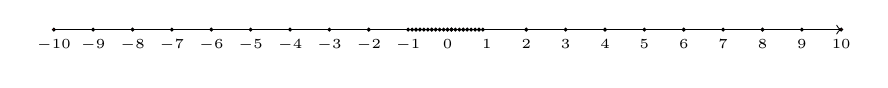
\begin{tikzpicture}[scale=0.5]
\foreach \x in {-10.0, -9.0, -8.0, -7.0, -6.0, -5.0, -4.0, -3.0, -2.0,
                -1.0, -.9, -.8, -.7, -.6, -.5, -.4, -.3, -.2, -.1, 0,
                .1, .2, .3, .4, .5, .6, .7, .8, .9, .10,
                2.0, 3.0, 4.0, 5.0, 6.0, 7.0, 8.0, 9.0, 10.0}
	{\draw[fill=red] (\x, 0) node[below] {} circle(1pt);};
\foreach \x in {-10, -9, -8, -7, -6, -5, -4, -3, -2,
                -1, 0, 1,
                2, 3, 4, 5, 6, 7, 8, 9, 10}
	{\node[below] at (\x, 0) {\tiny $\x$};};

\draw[->] (-10.0, 0) -- (10.0, 0);
\end{tikzpicture}
\end{itemize}
\end{frame}


\begin{frame}{Error bounds on floating point numbers}
Theorem: $|x - \fl(x)| \leq \half |x| \beta^{1-t} p$
where $p=1$ for rounding and $p=2$ for chopping.

Proof: Since $x = (\pm 0.\alpha_1 \alpha_2 \ldots \alpha_t \ldots) \beta^m$, we have
$\beta^{m-1} \leq |x| \leq \beta^m$. In the interval $[\beta^{m-1}, \beta^m]$, the floating point numbers
are evenly spaced with spacing $\beta^{m - t}$. Thus, for chopping,
\begin{equation*}
|x - \fl(x)| \leq \beta^{m - t} = \frac{p}{2} \beta^{m-t}, \text{ (with $p = 2$)}
\end{equation*}
and for rounding
\begin{equation*}
|x - \fl(x)| \leq \beta^{m - t} = \frac{p}{2} \beta^{m-t}, \text{ (with $p = 1$)}.
\end{equation*}
Hence
\begin{equation*}
|x - \fl(x)| \leq \frac{p}{2} \beta^{m - t} \leq \frac{p}{2} \beta^{1-t} \beta^{m-1} \leq \half |x| \beta^{1-t} p,\text{ independent of $m$}.
\end{equation*}
\end{frame}


\begin{frame}{Error bounds on floating point arithmetic}
Remark: $\delta = \frac{p}{2} \beta^{1-t}$ is called the unit roundoff error.\\
Let $\epsilon = \frac{\fl(x) - x}{x}$. Then $\fl(x) = (1 + \epsilon) x$, where $|\epsilon| \leq \delta$.\\
Theorem: Let $\odot$ denote the operation $+, -, \times \text{ or } \div$, and let $x$ and $y$ be
floating point numbers. Then
\begin{equation*}
\fl(x \odot y) = (x \odot y)(1 + \epsilon), \text{ where } |\epsilon| \leq \delta = \frac{p}{2} \beta^{1-t}.
\end{equation*}
Proof: By the previous theorem,
\begin{equation*}
|x \odot y - \fl(x \odot y)| \leq |x \odot y| \frac{p}{2} \beta^{1-t}.
\end{equation*}
Thus, $-|x \odot y| \frac{p}{2} \beta^{1 - t} \leq -x \odot y + \fl(x \odot y) \leq \frac{p}{2} \beta^{1 - t} |x \odot y|$.
Hence
\begin{equation*}
(x \odot y)\left(1 - \frac{|x \odot y|}{x \odot y} \beta^{1-t} \right) \leq \fl(x \odot y) \leq 
(x \odot y)\left(1 + \frac{|x \odot y|}{x \odot y} \beta^{1-t}\right).
\end{equation*}
It follows that $\fl(x \odot y) = (1 + \epsilon) (x \odot y)$ where
$|\epsilon| \leq \frac{p}{2} \beta^{1-t} = \delta$.
\end{frame}


\begin{frame}{Floating point addition for two or three summands}
\begin{equation*}
\begin{array}{rl}
\fl(x_1 + x_2) &= \fl(\fl(x_1) + \fl(x_2)) = \fl[x_1(1 + \hat{\epsilon_1)}) + x_2(1 + \hat{\epsilon_2})] \\
&= [x_1 (1 + \hat{\epsilon_1}) + x_2 (1 + \hat{\epsilon_1})] (1 + \epsilon),
\end{array}
\end{equation*}
where
$|\hat{\epsilon_1}| \leq \delta$, $|\hat{\epsilon_2}| \leq \delta$ and $|\epsilon_1| \leq \delta$. Similiarly,
\begin{equation*}
\begin{array}{rll}
\fl(x_1 + x_2 + x_3) &= ((&x_1 (1 + \hat{\epsilon_1})\\
&\qquad + &x_2 (1 + \hat{\epsilon_2}))(1 + \epsilon_1)\\
&\qquad +  &x_3 (1 + \hat{\epsilon_3})(1 + \epsilon_2) \\
& = (&x_1 (1 + \hat{\epsilon_1}) (1 + \epsilon_1) (1 + \epsilon_2) \\
	&\qquad + &x_2 (1 + \hat{\epsilon_2}) (1 + \epsilon_1) (1 + \epsilon_2)) \\
	&\qquad + &x_3 (1 + \hat{\epsilon_3}) (1 + \epsilon_2)
\end{array}
\end{equation*}
\end{frame}


\begin{frame}{Generalising to n terms}
Continuing this procedure,
\begin{equation*}
\begin{array}{rll}
\fl(\sum_{i=1}^n x_i) =& &x_1 (1 + \hat{\epsilon_1}) \prod_{i=1}^{n-1} (1 + \epsilon_i) \\
& + &x_2 (1 + \hat{\epsilon_2}) \prod_{i=1}^{n-1} (1 + \epsilon_i) \\
& + &x_3 (1 + \hat{\epsilon_3}) \prod_{i=2}^{n-1} (1 + \epsilon_i) \\
& + &x_4 (1 + \hat{\epsilon_4}) \prod_{i=3}^{n-1} (1 + \epsilon_i) \\
& + &\ldots + x_n (1 + \hat{\epsilon_n}) (1 + \epsilon_{n-1}) \\
&=& \sum_{i=1}^n [x_i (1 + \hat{\epsilon_i}) \prod_{j=1}^{n-1} (1 + \epsilon_j)].
\end{array}
\end{equation*}
Conclusion: 
\begin{itemize}
\item Floating point addition does not commute. Neither does any other floating point
			operation.
\item Hence the floating point numbers do not form a field.
\item To reduce rounding error, a sequence should be summed from small numbers to large numbers on a
computer.
\end{itemize}
\end{frame}


\begin{frame}{Here's what happens when you don't pay attention to such issues}
\begin{figure}
\caption{Would you like noise with that? Good luck finding the minimum.}
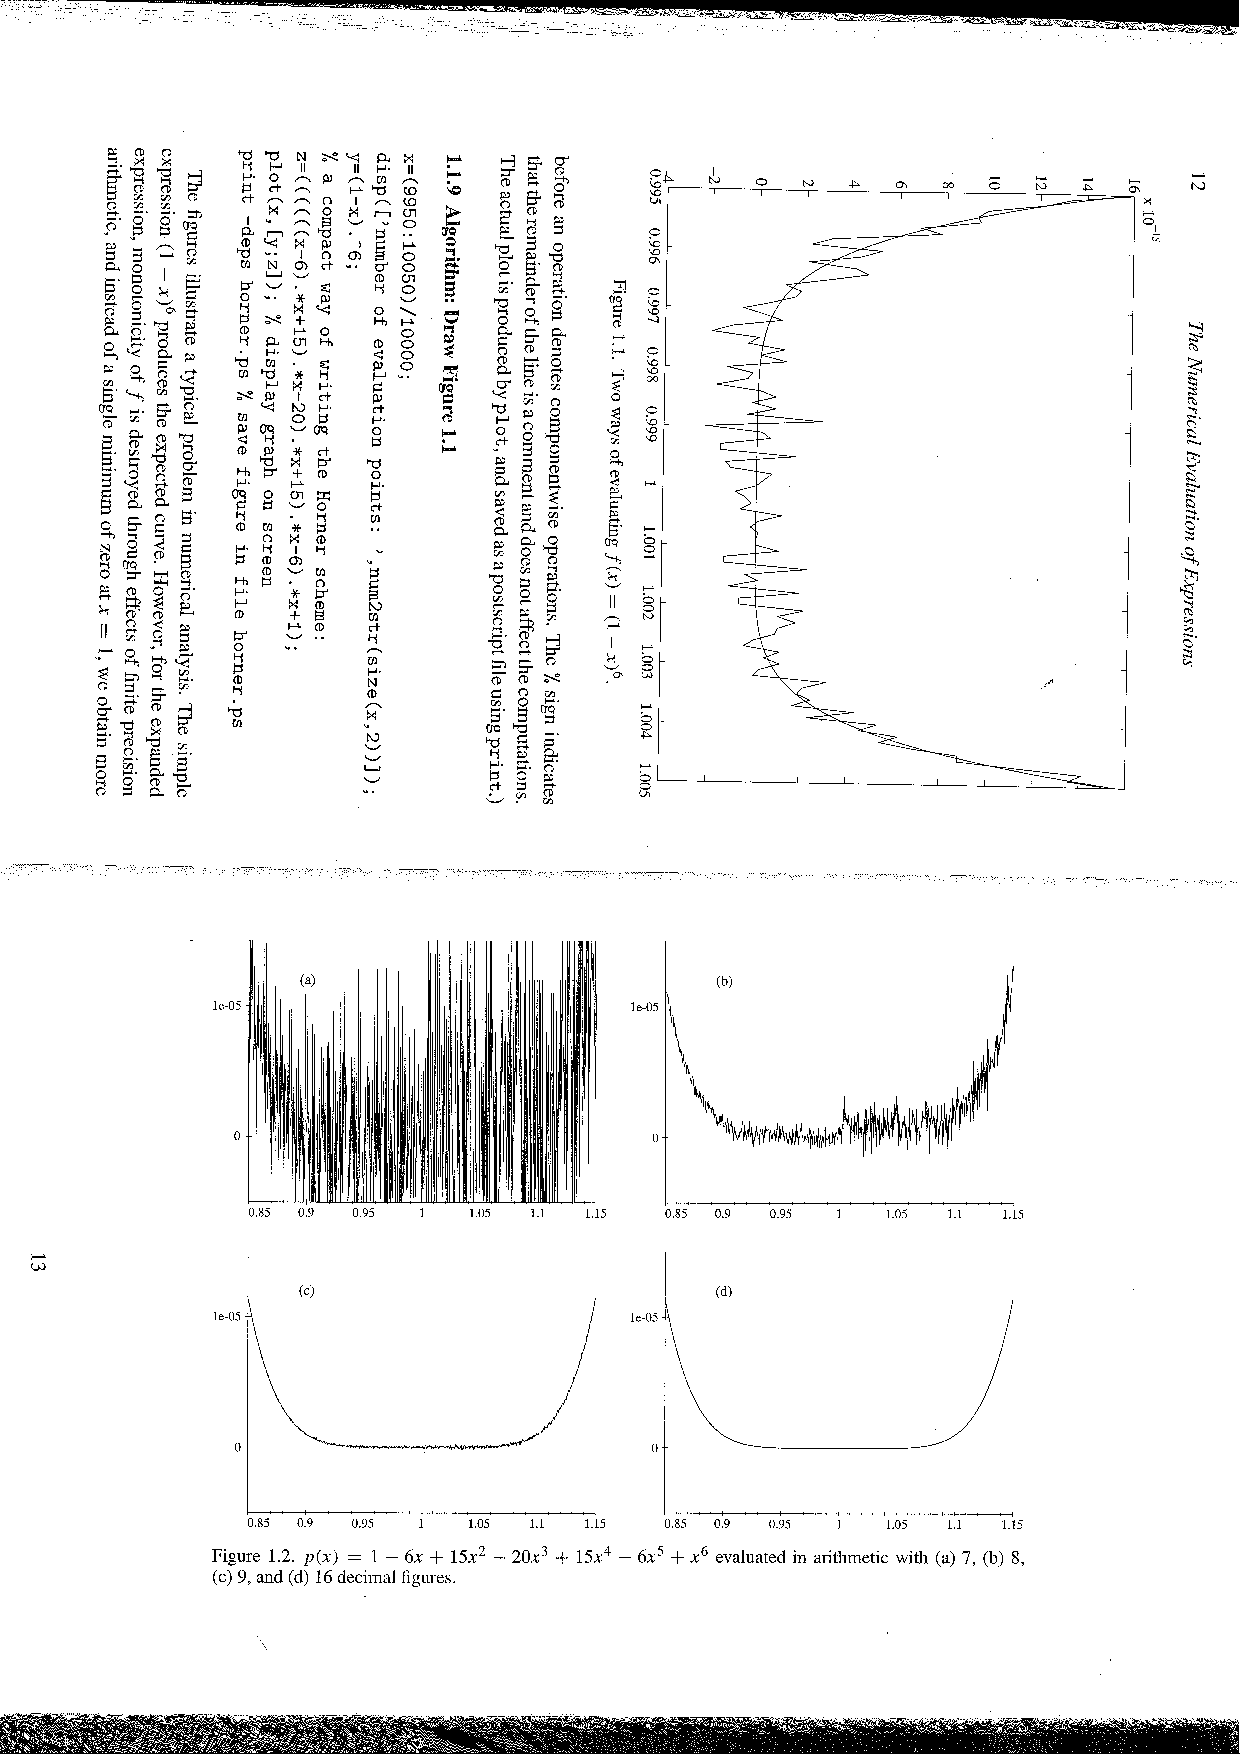
\includegraphics[scale=0.3, angle=91]{polynomial_evaluation.pdf}
\end{figure}

\end{frame}

\begin{frame}{Alternatives to floating point: more precision or arbtitrary precision}
\begin{itemize}
\item The easy answer is to throw more bits at the problem for more precision. Rather than single precision 				floating point, why not double? Or quadruple aka double double? Or double double double? Or, well, you 				get the idea \ldots
\item Another alternative from a conceptual standpoint is arbitrary precision, where numbers don't have to be
			stored in a fixed amount of memory.
\item Or just use rational numbers. $\mathbb{Q}$ is dense in $\mathbb{R}$.
\item Just keep computing with more digits until you reach the desired level of accuracy.
			\note{You could do this with streaming.}
\item Questions: If we can vary the number of digits we use, how many digits should that be? For a certain
			level of precision, how many are enough? When should our computations stop?
\note{From a numerical point of view, these are hard questions.}
\end{itemize}
\end{frame}


\begin{frame}{Continued fractions}
\begin{itemize}
\item Another idea some people have is to use continued fractions.
\item 
{\tiny
\text{Let }$x^2 &= 2$. Then
\begin{equation*}
\begin{array}{ll}
x^2 - 2 &= 0  \\
x^2 - 1 &= 1 \\
(x - 1)(x + 1) &= 1 \\
(x - 1)[2 + (x - 1)] &= 1 \\
x - 1 &= \frac{1}{2 + (x - 1)} \\
&= \frac{1}{2 + \frac{1}{2 + (x - 1)}} \\
&= \frac{1}{2 + \frac{1}{2 + \frac{1}{2 + \ldots}}}
\end{array}
\end{equation*}
So $x = 1 + \frac{1}{2 + \frac{1}{2 + \ldots}}$
}
\item For brevity, the ones are omitted except for the leading one and only the two's are notated.
			The above infinite continued fraction would be written $[1; 2, 2, 2, \ldots]$.
\end{itemize}
\end{frame}


\begin{frame}{Continued fractions continued}
\small
\begin{itemize}
\item Bill Gosper of MIT came up with algorithms to perform ``exact'' arithmetic on continued fractions in 
			1972.
\item You can move between continued fraction, power series and rational function representations of 
			functions.
\item The continued fraction representation of a function can converge more quickly than the power series 
			representation. And you only need to supply terms as they are needed.
\item \emph{Problem}: Calculating the square root of two is all very well. What happens when you try to go
			the other way? What is $\sqrt{2} \times \sqrt{2} = [1; 2, 2, 2, \ldots] \times [1; 2, 2, 2, \ldots]$?
\item Gosper'’s mul­ti­plica­tion scheme will run for­ever with­out return­ing a sin­gle number, because whether the
			first number is 2 or 1 depends on all of the infi­nite preci­sion in the operands.
\item People like Peter Potts propose fixes for this like nested linear fractional transformations and
			redundant binary digit encoding. I thought this approach was supposed to be \emph{simpler}?
\item Not likely to be implemented in silicon any time soon \ldots
\end{itemize}
\end{frame}

% <StyxAlso> edwardk, Possibly dumb question about continued fractions.
% <StyxAlso> http://www.cs.virginia.edu/~lat7h/blog/posts/7.html makes the point that multiplication need not terminate e.g. sqrt(2) * sqrt(2)
% <StyxAlso> edwardk, How do you get around this?
% <spacekitteh> laziness, presumably?
% <StyxAlso> I don't think so in this case
% <StyxAlso> The problem is that sqrt(2) has an infinite continued fraction representation
% <erikd> StyxAlso: edwardk is on the east coast of the US, where its currently 5 am
% <StyxAlso> Until you get to the "last" digit, you don't know whether you have the square root of two or not
% <StyxAlso> So you don't know whether to output the first digit of your result as a 1 or a 2. And can't know.
% <StyxAlso> erikd, Okay. An answer tomorrow is fine by me.
% <StyxAlso> This is using Bill Gosper's algorithms unmodified. If there's a way out of this trap, I'd like to know about it.
% <StyxAlso> Even if continued fractions aren't the right solution for everything, they're very interesting and useful for some things.
% <StyxAlso> My supervisor wrote a paper on using them to evaluate special functions.
% <pjdelport> StyxAlso: One approach that gets used is narrowing intervals, I think.
% <StyxAlso> Yes. Which is quite different. Closer in spirit to floating point.
% <pjdelport> http://www.tweedledum.com/rwg/cfup.htm also talks about it in the context of using continued logarithms (search down for ".999... problem")
% <StyxAlso> I expected the problem was known. I was hoping that it was also solved.
% <pjdelport> Jean Vuillem­in's "Exact Real Com­puter Arithmetic with Con­tin­ued Frac­tions" paper also addresses it, I think.
% * erikd has quit (Read error: Connection timed out)
% * erikd (~erikd@hendrix.mega-nerd.net) has joined #haskell.au
% * brenton (uid39276@gateway/web/irccloud.com/x-tkavmaszyslgmbgh) has joined #haskell.au
% * michaelneale has quit (Quit: Back later)
% <edwardk> erikd: he also doesn't sleep much
% <edwardk> StyxAlso: this is why continued fractions break down and you need nested linear fractional transformations
% <StyxAlso> Right.
% <StyxAlso> Do you have a reference? Perhaps you've already provided me with one.
% <edwardk> StyxAlso: then you can do things like switch to a different 'digit' matrix representation that can make progress
% <edwardk> e.g. redundant binary
% <edwardk> peter potts' thesis uses a redundant binary digit encoding
% <erikd> edwardk: wow! if i don't get 6-7 solid hours, i'm completely useless!!!
% <StyxAlso> edwardk, I take it this isn't going to be implemented in silicon any time soon.
% <StyxAlso> Sounds complicated.
% <edwardk> unlikely =)
% * StyxAlso chuckles.

\begin{frame}{More exotic alternatives: UNums 2.0}
\begin{itemize}
\item Key idea: Lose precision gradually and gracefully, rather than suddenly like floating point.
\item Based on the stereographic projection of the real line to the unit circle. 
% \begin{tikzpicture}[
%     x                = 2cm/10,
%     scale            = 3,
%     axis/.style      = {help lines, -{Stealth[length = 1.5ex]}},
%     brillouin/.style = {domain = -5:10, samples = 100}
%   ]
%   \draw [axis] (-5,0) -- (10,0);
%   \draw [axis] (0,-1) -- (0,1.5);
%   \draw [densely dotted] (0,{ Unum_fun(100)} ) -- ++(10,0);
%   \draw [red]   plot [Unum] (\x, { Brillouin(\x)});
%   \draw [green] plot [brillouin] (\x, { Brillouin(5,  \x)});
%   \draw [blue]  plot [brillouin] (\x, { Brillouin(50, \x)});
%   \node [align = center, anchor = west] at (1,1.3) {%
%     $\begin{alignedat}{2}
%       B_J(x) &= \tfrac{2J + 1}{2J}
%                 &&\coth \left ( \tfrac{2J + 1}{2J} x \right ) \\
%              &\quad - \tfrac{1}{2J}
%                 &&\coth \left ( \tfrac{1}{2J} x \right )
%      \end{alignedat}$};
% \end{tikzpicture}
% TODO: Prepare this picture.
\item Let $f(x) = \frac{x}{1 + |x|}$. Clearly $f: (-\infty, \infty) \to (-1, 1)$ and is a bijection.
\item Then apply the map $x \mapsto e^{i \pi x} + i$.

\begin{minipage}{\textwidth}\centering
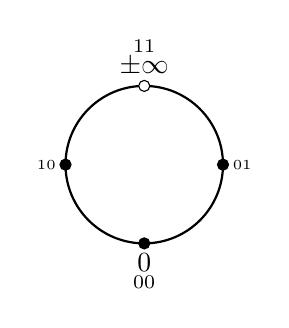
\begin{tikzpicture}
\draw[thick] (0cm,0cm) circle(1cm);
\draw[fill=black] (0cm, -1cm) node[below] {$\underset{00}{0}$} circle(2pt);
\draw[fill=black] (1cm, 0cm) node[right] {\tiny $01$} circle(2pt);
\draw[fill=black] (-1cm, 0cm) node[left] {\tiny $10$} circle(2pt);
\draw[fill=white] (0cm, 1cm) node[above] {$\overset{11}{\pm \infty}$} circle(2pt);
\end{tikzpicture}
\end{minipage}

\item Real part is x, imaginary part is y.
\end{itemize}
\end{frame}


\begin{frame}{Fingers crossed we might see this in hardware one day!}
\begin{itemize}
\item Professor John Gustaffson, ex-Intel, author of ``The End of Error: Unum Computing'',
			already superceded (!).
\item Very new, presented at Multicore World 2016.
\item He has a plan for how to get this into hardware.
\item Check out his PowerPoint presentation.
\item A little bird tells me that Intel finds this interesting, and ``may look at implementing this in
			six year's time.''. They refused to be quoted!
\end{itemize}
\end{frame}


\begin{frame}{There's no silver bullet. Better the devil you know?}
\begin{itemize}
\item Floating point arithmetic is ubiquitous, like QWERTY or (insert thing
			you don't like here). It's implemented in hardware you can buy today and it is well understood.
\item We have centuries of numerical analysis from which to draw when analysing the error in our algorithms.
			Changing representations means at least partially abandoning that.
\item Beware the Wrath of Kahan: alternatives often end up suffering from the same shortcomings. 
			William Kahan aka the Father of floating point arithmetic, enjoys pointing this out.
\item A few clock cycles is about as long as I care to wait for numerics. Or anything, really \ldots
\item Serious answer: Use the right representation in the right situation. But know what price you're 
			paying, and how much precision you're really getting.
\end{itemize}
\end{frame}


\begin{frame}{Acknowledgements/Questions?}
\begin{itemize}
\item My PhD supervisor Dr John Ormerod, for setting me a problem which drove me to learn about these
			issues, for the numeric inspiration and for introducing me to continued fractions.
\item My Honours supervisor Dr Daniel Daners for inspiring my love of mathematical analysis and teaching
			me how to write proofs.
\item Charles Gray from Latrobe for TikZ help and presentation advice.
\item Dr Danya Rose from USyd for suggestions on how the proofs could be made more clear, and TikZ help.
\item Liam O'Connor from UNSW, for stimulating conversations on foundational issues.
\item Thomas Sutton for proof reading, and making helpful suggestions.
\item Erik de Casto Lopo, for being such a fine intellectual sparring partner all these years.
\item Any questions?
\end{itemize}
\end{frame}

% edwardk> StyxAlso: hakmem
% <edwardk> http://www.inwap.com/pdp10/hbaker/hakmem/cf.html#item101b
% <edwardk> mvr_ can probably give you an exhaustive set of references as well
% <edwardk> khinchin's book on continued fractions is a good reference: http://www.amazon.com/Continued-Fractions-Dover-Books-Mathematics/dp/0486696308
% <edwardk> mjd has a quick implementation of continued fractions in perl and associated talk here: http://perl.plover.com/yak/cftalk/ but be warned the variable order differs from all the other presentations
% <edwardk> peter potts' ph.d thesis on continued fractions did a lot to inform my thinking as well: http://peterpotts.com/arithmetic.html
% <edwardk> from that thesis you can find other links in the bibliography
% <mvr_> StyxAlso: this is the longer brief on continued fractions by bill gosper: http://perl.plover.com/yak/cftalk/INFO/gosper.txt
% <edwardk> StyxAlso: that should cover 90% of the stuff i care about
% <edwardk> yeah that is a better gosper writeup

\end{document}
